%%%%%%%%%%%%%%%%%%%%%%%%%%%%%%%%%%%%%%%%%%%%%%%%%%%%%%%%%%%%%%%%%%%%%%%%%%%%%%
%
% PRÉAMBULE
%
%

% LaTeX 2e sinon rien !
\NeedsTeXFormat{LaTeX2e}

% C'est un rapport...
\documentclass[a4paper,11pt]{report}

% Style du document : personnalisé si disponible, sinon LaTeX par défaut
\IfFileExists{bglstyle.sty}{
  \usepackage{bglstyle} % Mon identité visuelle ;-)
}{
  % Packages de base
  \usepackage[utf8]{inputenc}
  \usepackage[T1]{fontenc}
  \usepackage{textcomp,ae,aecompl,aeguill}
  \usepackage[margin=3cm]{geometry}

  % Commandes définies ici pour assurer la compatibilité avec le style perso
  \makeatletter
  \renewcommand{\title}[1]{\renewcommand{\@mytitle}{#1}}
  \newcommand{\@mytitle}{}
  \newcommand{\subtitle}[1]{\renewcommand{\@title}{\@mytitle\\#1}}
  \newcommand{\group}[1]{}
  \newcommand{\entity}[1]{}
  \makeatother

  % Si jamais le rendu du style LaTeX standard diffère légèrement du style
  % personnalisé, ça ne produira pas d'avertissement (overful/underful hbox)
  \sloppy
}

% Packages supplémentaires utilisés par ce document
\usepackage{graphicx,multicol}
\usepackage[french,english]{babel}

% Hyperlinks
\ifpdf
  \usepackage[pdftex,bookmarks,bookmarksopen,bookmarksnumbered,%
              pdfstartview=Fit,pdfview=Fit]{hyperref}
  \makeatletter
  \hypersetup{%
    pdftitle    = {\@title},
    pdfauthor   = {\@author},
    pdfborder   = {0 0 0}
  \makeatother
}
  \usepackage{thumbpdf}
\else
  \usepackage[dvips]{hyperref}
\fi

% Commandes personnalisées
\newcommand{\ensp}[1]{\selectlanguage{english}#1\selectlanguage{french}}
\newcommand{\strong}[1]{\textbf{#1}}
\newcommand{\file}[1]{\ensp{\textsf{#1}}}
\newcommand{\var}[1]{\ensp{\textit{#1}}}
\newcommand{\type}[1]{\ensp{\texttt{#1}}}
\newcommand{\class}[1]{\ensp{\textsf{#1}}}

% Informations sur le document
\title{%
  {\large Théorie des Langages et Compilation}\\
  Lecteur de configuration\\de pare-feu%
}
\subtitle{Rapport}
\author{Benjamin \textsc{Gaillard}}
\date{16 janvier 2006}
\group{Master 1 RIA --- Groupe 2}
\entity{\includegraphics[keepaspectratio,height=1.5cm]{images/ulp}}


%%%%%%%%%%%%%%%%%%%%%%%%%%%%%%%%%%%%%%%%%%%%%%%%%%%%%%%%%%%%%%%%%%%%%%%%%%%%%%
%
% CONTENU (enfin !)
%
%

\begin{document} % Pas d'indentation pour cet environnement de base

\selectlanguage{french}
\maketitle
\tableofcontents

\chapter*{Introduction}
\markboth{Introduction}{Introduction}
\addcontentsline{toc}{chapter}{Introduction}

Le but de ce projet est de développer un logiciel en C, Lex et Yacc capable de
lire, d'afficher et de transformer en règles IPTables une configuration de
pare-feu dont la syntaxe est définie dans le sujet ainsi que de concevoir une
extension élargissant le champ d'application du langage.

Dans ce rapport, nous allons donc décrire la grammaire utilisée pour le
langage de base présenté dans le sujet, suivie de la description des valeurs
sémantiques associées à chaque symbole et des structures de données qui sont
employées à cette fin. Nous présenterons finalement l'extension apportée au
langage ainsi que le mécanisme utilisé pour transformer une telle
configuration en un ensemble de commandes IPTables, sans oublier, pour
terminer, quelques détails techniques sur l'implémentation de ce projet.

\chapter{Grammaire du langage de base}

\begin{intro}
  Dans cette partie est présentée la grammaire établie pour le langage de base
  décrit dans le sujet. C'est à partir de cette description formelle que Yacc
  (ou Bison, la version GNU) pourra générer un analyseur syntaxique en C.
\end{intro}

La syntaxe utilisée dans les fichier pour Yacc est assez explicite, et suffit
pour décrire formellement la grammaire du langage de base utilisée. Les
symboles sont assez explicites ; ceux en majuscules sont terminaux
(c'est-à-dire reconnus par l'analyseur lexical), les autres sont traités par
Yacc.

Voici donc une version de ce fichier vidée de son code C :

{\small\begin{verbatim}
/* A configuration: a chain ensemble */
configuration
    : chain configuration
    | chain;

/* A chain definition */
chain
    : NEWCHAIN ASSIGN action CHAINSEP;

/* An action : final, user or conditional (test) */
action
    : FINAL
    | test;

/* An if/then/else test */
test
    : IF expr test_then action ELSE action;
test_then: THEN | ;

/* A test expression */
expr
    : OP_NOT expr
    | PAR_OPEN expr PAR_CLOSE
    | expr OP_AND expr
    | expr OP_OR expr
    | condition;

/* A simple condition */
condition
    : IP direction addrs
    | PROTO direction ports;

/* A packet direction */
direction
    : DIRECTION
    | ;

/* Either a single address or an address list */
addrs
    : addr
    | LIST_BEGIN addrlist LIST_END;

/* An address list */
addrlist
    : addr LIST_SEP addrlist
    | addr;

/* One address */
addr
    : ADDR;

/* Either a single port or a port list */
ports
    : port
    | LIST_BEGIN portlist LIST_END;

/* A port list */
portlist
    : port LIST_SEP portlist
    | port;

/* One port */
port
    : PORT
    | PORTNAME;
\end{verbatim}}

\chapter{Valeur sémantique des symboles}

\begin{intro}
  Cette partie va nous servir à décrire à quoi correspondent sémantiquement
  les différents symboles utilisés dans notre grammaire, autrement dit ce
  qu'ils représentent par rapport au langage.
\end{intro}

\section{Symboles non terminaux}

\begin{description}
  \item[configuration et chain]~\\
    Ces deux symboles ont le même type, à savoir
    un pointeur sur une structure représentant une chaîne. Le premier,
    \emph{configuration}, est utilisé pour faire une liste chaînée de toutes
    les chaînes présentes dans la configuration. Une structure chaîne contient
    le nom de la chaîne ainsi qu'un pointeur vers la structure \emph{action}
    correspondante.

  \item[action]~\\
    Le type de ce symbole est un pointeur sur une structure
    représentant une action à effectuer, qui peut être soit un test soit une
    action finale. Dans les deux cas, il y a un pointeur vers la structure
    correspondant à chacun.

  \item[test]~\\
    Ce symbole représente le triplet \emph{if/then/else} ; son
    type est un pointeur vers une structure contenant trois pointeurs : le
    premier vers la structure \emph{test} correspondante, les deux autres
    vers les deux structures \emph{action} associées aux branches
    \og then\fg{} et \og else\fg.

  \item[expr]~\\
    Une expression est représentée à travers ce symbole. Ce sont les
    expressions qui composent une condition complexe : elle peut être soit
    un \emph{ET} logique, ou un \emph{OU} logique ou une condition simple.
    Quand il s'agit des opérateurs logiques, il y a deux pointeurs vers les
    expressions représentant les opérandes gauche et droite. Dans le troisième
    cas, il s'agit bien sûr d'un pointeur vers une structure
    \emph{condition}.\\
    Dans tous les cas, un booléen indique si la condition doit être inversée
    ou pas (négation). Cela a deux avantages : tout d'abord on peut
    s'affranchir de devoir gérer un opérateur supplémentaire de négation ;
    ensuite, il est très facile de gérer les cas de négation multiple
    puisqu'il suffit alors d'inverser plusieurs fois ce booléen.

  \item[condition]~\\
    Le symbole \emph{condition} sert à définir une condition simple,
    c'est-à-dire un test sur les adresses ou les ports. La structure utilisée
    contient quatre champs principaux : le premier indique s'il s'agit d'un
    test sur les adresses ou les ports ; le second indique le protocole
    associé (IPv4 ou IPv6 --- finalement non implémenté, voir le chapitre
    traitant de l'extension ---, TCP ou UDP), le troisième la direction
    (source, destination, les deux) et le quatrième est un pointeur vers la
    structure \emph{addr} ou \emph{port} associée.

  \item[direction]~\\
    Ce symbole correspond exactement au symbole terminal ayant la même
    fonction, seulement il gère le cas où la direction est omise, auquel cas
    on pourra indiquer que les deux sens sont à traiter. Le type correspondant
    est une énumération des trois directions possibles (source, destination,
    les deux).

  \item[addrs, addrlist et addr]~\\
    Ces trois symboles représentent une adresse ou une liste d'adresses. Le
    type est le même pour les trois, à savoir un pointeur vers une structure
    \emph{addr}. Seulement, \emph{addrs} peut être à la fois une adresse
    unique ou une liste ; et une liste est délimitée et composée de plusieurs
    adresses uniques, le symbole \emph{addrlist} permettant ainsi de les lier
    entre elles sous forme de liste chaînée. Une adresse unique est
    représentée par une chaîne de caractères.

  \item[ports, portlist et port]~\\
    Il s'agit ici exactement du même principe que les adresses, mais appliqué
    aux ports. Un port unique peut être soit un port simple, un intervalle de
    ports ou un nom de port.
\end{description}

\section{Symboles terminaux}

\subsection{Définition des chaînes}

\begin{description}
  \item[ASSIGN et CHAINSEP]~\\
    Ils correspondent simplement aux opérateurs \og=\fg{} et \og\ensp{;}\fg{}
    respectivement, et n'ont pas de type.

  \item[NEWCHAIN]~\\
    De type chaîne de caractères, cela correspond au nom de la chaîne.

  \item[FINAL]~\\
    Cela définit une \og action finale\fg, à savoir l'une parmi \emph{accept},
    \emph{drop} et \emph{reject}. Le type employé est une énumération.
\end{description}

\subsection{Condition}

\begin{description}
  \item[IF, THEN et ELSE]~\\
    Ces symboles représentent les mots-clés \emph{if}, \emph{then} et
    \emph{else}. Il n'y a pas de type associé à ces symboles.

  \item[PAR\_OPEN et PAR\_CLOSE]~\\
    Les parenthèses respectivement ouvrante et fermante sont représentées par
    ces symboles, qui n'ont également pas de type.

  \item[OP\_OR, OP\_AND et OP\_NOT]~\\
    Ces symboles-là sont utilisés pour représenter les trois opérateurs
    logiques employés dans les expressions conditionnelles : \emph{OU},
    \emph{ET} et \emph{NON}. Eux non plus n'ont pas de type. Leur ordre
    de priorité, tel que présenté ici, est du moins au plus propritaire. Les
    deux opérateurs binaires sont, par convention, associatifs à gauche.
\end{description}

\subsection{Protocole}

\begin{description}
  \item[IP et PROTO]~\\
    Le protocole réseau (IP) et le protocole transport (TCP, UDP) sont
    associés à ces symboles. Leur type est une énumération de tous les
    protocoles employés dans cette grammaire.

  \item[DIRECTION]~\\
    Il s'agit de la même chose que le symbole non terminal du même nom (la
    direction des paquets étudiée) et le type est identique, à savoir une
    énumération des trois options possibles.
\end{description}

\subsection{Liste}

\begin{description}
  \item[LIST\_BEGIN, LIST\_END et LIST\_SEP]~\\
    Il s'agit ici des symboles représentant les trois opérateurs utilisés pour
    créer une liste, respectivement : début de liste, fin de liste, et
    opérateur de séparation des éléments. Ils n'ont pas de type.
\end{description}

\subsection{Adresse}

\begin{description}
  \item[ADDR]~\\
    C'est le symbole utilisé pour représenter une adresse. Le type
    correspondant est une chaîne, quel que soit le type de l'adresse (IP
    numérique, DNS, postfixé ou pas d'un masque\dots). C'est l'analyseur
    lexical qui est chargé de les reconnaître correctement. En effet, dans la
    plupart des utilisations que l'on pourrait faire de cette grammaire, il
    n'est pas utile de différencier les types d'adresses.
\end{description}

\subsection{Port}

\begin{description}
  \item[PORT]~\\
    Ce symbole représente un port donné de façon numérique, soit sous forme
    de port unique soit sous la forme d'un intervalle. Dans les deux cas, le
    type utilisé est une structure contenant deux champs : le début et la fin
    de l'intervalle. Dans le cas d'un port unique, ces deux champs contiennent
    la même valeur.

  \item[PORTNAME]~\\
    Un port écrit sous forme de nom est représenté par ce symbole. Le type
    employé est naturellement une chaîne de caractères.
\end{description}

\subsection{Symbole invalide}

\begin{description}
  \item[INVALID]~\\
    Ce symbole ne représente rien en particulier ; il est seulement utilisé
    pour désigner une erreur lexicale (et donc grammaticale puisqu'il
    n'apparaît dans aucune des règles grammaticales).
\end{description}
%token INVALID

\chapter{Structures de données}

\begin{intro}
  Les structures de données utilisées pour stocker la configuration lue va
  être présentée dans cette partie. Il s'agit d'une étape importante, car
  elles permettent non seulement de mémoriser les entrées, mais c'est
  également sur elles que seront effectués les traitements en vue de leur
  exploitation.
\end{intro}

\section{Description formelle}

Les structures utilisées dans ce projet correspondent exactement aux symboles
grammaticaux (non terminaux donc). À chaque symbole sa structure, sauf bien
sûr dans les cas où plusieurs symboles utilisent la même structure pour
construire des listes (chaînes, adresses et ports).

Il n'est donc point besoin de redécrire ce qui l'a déjà été, puisque les mêmes
remarques s'appliquent ici également. Nous allons donc directement présenter
les structures telles qu'elles ont été définies en langage C. Laissons donc
parler le C, et voici, ci-dessous, les sus-dites déclarations.

{\small\begin{verbatim}
/*
 * Custom types: enumerations
 */

/* Boolean value */
enum bool { FALSE = 0, TRUE = 1 };

/* Final target */
enum final { FINAL_ACCEPT, FINAL_DROP, FINAL_REJECT };

/* Expression type */
enum expr_type { EXPR_COND, EXPR_AND, EXPR_OR };

/* Type of condition */
enum cond_type { COND_ADDR, COND_PORT };

/* Protocols */
enum proto { PROTO_IP = 0, PROTO_IPV4, PROTO_IPV6,
             PROTO_PORT, PROTO_TCP, PROTO_UDP };

/* Packet direction */
enum direction { DIR_BOTH, DIR_SRC, DIR_DST };

/* A port range */
struct one_port { unsigned short from, to; };


/*
 * Custom types: structures
 */

/* Chain */
struct chain {
    struct chain *next;    /* Next chain (linked list) */
    char *name;            /* Chain name               */
    struct action *action; /* Associated action        */
};

/* Action */
struct action {
    enum { TARGET_FINAL, TARGET_USER, TARGET_TEST } type; /* Action type */
    union {
        enum final          final; /* Final target       */
        const struct chain *user;  /* User-defined chain */
        struct test        *test;  /* Test (conditions)  */
    } action;
};

/* Test */
struct test {
    struct expr *expr;                  /* Associated test expression */
    struct action *act_then, *act_else; /* Taken actions              */
};

/* Expression */
struct expr {
    enum bool not;       /* Wether to negate test ("!" operator) */
    enum expr_type type; /* Expression type                      */
    union {
        struct {
            struct expr *left, *right; /* Left and right operands */
        } expr;
        struct condition *cond; /* Condition */
    } sub;
};

/* Condition */
struct condition {
    enum cond_type type; /* Condition type     */
    enum direction dir;  /* Packet direction   */
    enum proto proto;    /* Concerned protocol */
    union {
        struct addr *addr; /* Host address    */
        struct port *port; /* Port (TCP, UDP) */
    } cond;
};

/* Host address */
struct addr {
    struct addr *next; /* Next address (linked list) */
    char *string;      /* Corresponding string       */
};

/* Port number/range/name */
struct port {
    struct port *next;                     /* Next port range (linked list) */
    enum { PORT_NUMERIC, PORT_NAME } type; /* Port type                     */
    union {
        struct one_port range; /* Port range */
        char *name;            /* Port name  */
    } port;
};

\end{verbatim}}

\section{Schéma récapitulatif}

\begin{center}
  \noindent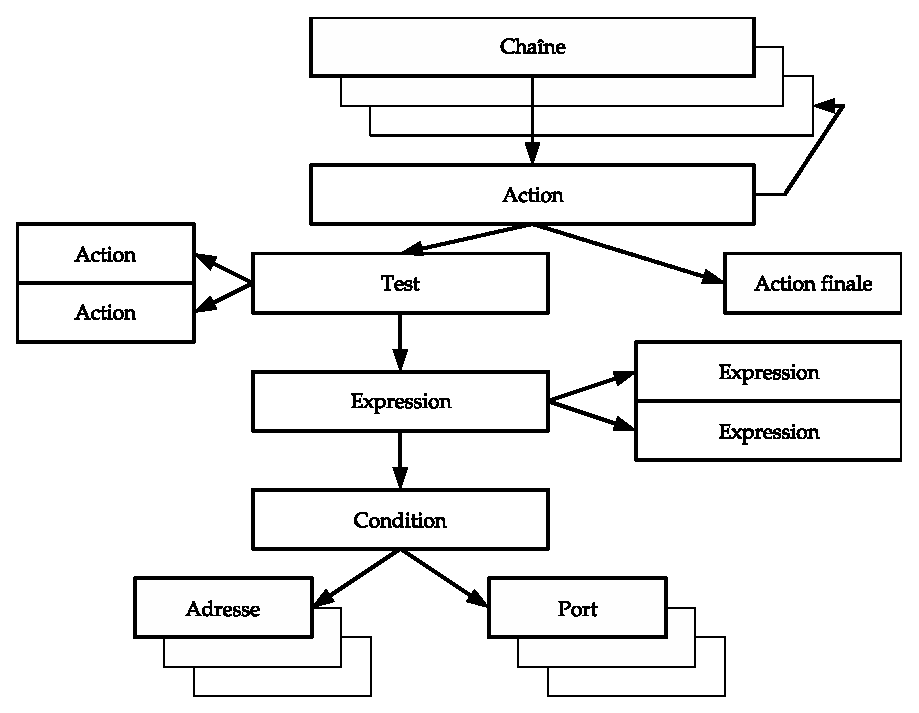
\includegraphics[keepaspectratio,width=0.9\textwidth]{schema}
\end{center}

\chapter{Extension du langage}

\begin{intro}
  Le langage tel que défini dans le sujet s'est vu étendu par quelques
  modifications qui lui ont été apportées. Nous allons décrire dans cette
  partie de quoi il en retourne exactement.
\end{intro}

\section{Mots-clés supplémentaires}

Certains mots-clés ont été ajoutés afin de rendre le langage plus utilisable
dans certains cas. Ces mots sont les suivants :

\begin{itemize}
  \item\strong{src} et \strong{dst} : ces deux mots peuvent être utilisés à
    la place de \emph{source} et \emph{destination}, pour une écriture plus
    rapide des tests ;
  \item\strong{both} : celui-ci a été rajouté pour explicitement indiquer que
    les deux directions doivent s'appliquer au test ; ceci peut être utile
    dans le cas où une machine s'appellerait \emph{source} ou
    \emph{destination} ;
  \item\strong{port} : ce mot est utilisé pour désigner à la fois TCP et UDP ;
  \item\strong{ACCEPT}, \strong{DROP} et \strong{REJECT} : ces trois
    \og actions finales\fg{} sont maintenant également acceptées en
    majuscules ;
  \item\strong{ipv4} et \strong{ipv6} : ces mots ont été ajoutés dans le
    lexique mais ne sont cependant pas reconnus par la grammaire ; voir
    ci-après la section sur IPv6 pour une explication.
\end{itemize}

\bigskip
Ces mots-clés supplémentaires n'ont aucun effet sur la grammaire elle-même,
seuls des changements dans le lexique ont été effectués. Quelques valeurs ont
également été rajoutées dans les énumérations.

\section{Commentaires}

Avec cette extension, il est mainteant possible d'inclure des commentaires
dans les fichiers de configuration. Trois types de commentaires sont
reconnus :

\begin{itemize}
  \item style shell : ils commencent par un dièse (\og\texttt{\#}\fg) et se
    terminent par un retour à la ligne ;
  \item style C++ : ils commencent par deux slashes (\og\texttt{//}\fg) et se
    terminent par un retour à la ligne ;
  \item style C : ils commencent par \og\texttt{/*}\fg{} et se terminent par
    \og\texttt{*/}\fg.
\end{itemize}

\bigskip
Cette extension n'a qu'une influence sur le lexique, et aucun autre fichier.

\section{Inclusions}

Au moyen de cette extension nous pouvons inclure d'autres fichiers dans la
configuration courante. Il faut, pour cela, entrer entre deux descriptions de
chaînes la ligne suivante :

\verb!include fichier! ou \verb!include "fichier"!

\bigskip
Le fichier est recherché relativement à la localisation du fichier incluant,
dans l'arborescence du système de fichiers.

Les changements engendrés par cette extension ne concernent que le lexique
uniquement, car il s'occupe seul de la lecture de l'entrée. Un système à base
de pile a été implémenté.

\section{Chaînes utilisateur}

Avec le langage d'origine, il était possible de définir des chaînes, mais cela
s'arrêtait là. Avec cette extension, il est maintenant possible de les
utiliser. Là où l'on peut mettre \emph{accept}, \emph{drop} ou \emph{reject},
on peut maintenant mettre le nom de n'importe quelle chaîne que l'on a déjà
définie. Attention cependant, il est invalide de faire référence à une chaîne
qui n'a pas encore été définie !

Avec cette extension, on se rapproche de l'implémentation usuelle des pare-feu
qui permettent de définir plusieurs chaînes ou tables. Cela permet en effet
une utilisation beaucoup plus poussée et plus souple de ce genre d'outils
puisqu'il est possible de porter des modifications à quelques chaînes
seulement sans avoir à réécrire toute la configuration.

Cette extension impose quelques changements dans le lexique (pour reconnaître
une chaîne utilisateur définie), dans les structures de données (un nouveau
type d'action avant un pointeur sur une structure \emph{chaîne}) ainsi que sur
la grammaire, devant maintenant prendre en compte un nouveau type d'action.
Les changements sont toutefois mineurs dans chaque cas.

\section{IPv6}

Cette extension était au départ prévue pour être intégrée dans le langage.
Cependant, pour des raisons de complications liées aux changements impliqués
dans les structures, à de nombreux tests supplémentaires et à de profondes
modifications dans les commandes IPTables générées, elle a été abansonnée.

C'est la raison pour laquelle certains symboles sont présents dans le lexique
ainsi que la présence d'éléments liés à IPv6 dans les structures de données
peuvent être remarqués dans les fichiers sources. Ils n'ont cependant pas été
retirés, en vue d'une hypothétique amélioration future du projet, et ne gênent
nullement dans leur état actuel.

\chapter{Règles IPTables}

\begin{intro}
  C'est dans cette partie que sera présentée la façon dont l'arbre
  représentant la configuration va être transformé en commandes IPTables.
\end{intro}

Une série de fonctions, implémentées dans le fichier \verb!iptables.c!, va
parcourir l'arbre du langage comme le font les fonctions d'affichage.
Seulement, évidemment, les traitements effectués ne sont pas du tout les
mêmes. Voici une description de l'algorithme employé :

\begin{itemize}
  \item Pour chaque chaîne utilisateur, une chaîne IPTables correspondante est
    créée.
  \item Pour une action finale (\emph{accept}, \emph{drop}, \emph{reject}),
    un saut vers les équivalents IPTables (respectivement \emph{ACCEPT},
    \emph{DROP}, \emph{REJECT}) est effectué.
  \item Pour une action \og chaîne utilisateur\fg, de la même manière, un saut
    est effectué vers la chaîne IPTables correspondante.
  \item En cas de test, là, ça devient plus compliqué :
  \begin{itemize}
    \item Deux tables sont créées, une pour chaque branche de la condition.
    \item Ensuite, l'algorithme suivant est exécuté pour chaque expression de
      la condition :
    \begin{itemize}
      \item Si l'expression comporte une négation (booléen dont il était
	question plus haut dans ce rapport), les deux branches (tables) sont
	inversées.
      \item Si l'expression est un ET ou un OU logique, on crée une table
	intermédiaire.
      \item Dans le cas d'un ET :
      \begin{itemize}
	\item On applique l'algorithme de l'expression sur l'opérande de
	  gauche sur la table actuelle, avec comme branche positive la table
	  intermédiaire et comme branche négative la branche négative
	  actuelle.
      \end{itemize}
      \item Dans le cas d'un OU :
      \begin{itemize}
	\item On applique l'algorithme de l'expression sur l'opérande de
	  gauche sur la table actuelle, avec comme branche positive la branche
	  positive actuelle et comme branche négative la table intermédiaire.
      \end{itemize}
      \item On applique l'algorithme de l'expression sur l'opérande de
	droite sur la table intermédiaire, avec comme branche positive la
	branche positive actuelle et comme branche négative la branche
	négative actuelle.
    \end{itemize}
    \item Maintenant, dans le cas d'un condition simple, chaque élément est
      testé un à un (chaque adresse dans chaque direction, chaque port pour
      chaque protocole pour chaque direction). Des règles IPTables sont
      générées sur la table actuelle de telle sorte que lorsque le test est
      positif, un saut est effectué vers la branche positive. À la fin des
      tests, un saut inconditionnel est effectué vers la branche négative.
  \end{itemize}
\end{itemize}

\bigskip
Voici grosso-modo la façon dont fonctionne la transformation. Contrairement à
un compilateur plus traditionnel, aucun traitement particulier n'est appliqué
à l'arbre du langage. Il est simplement parcouru en employant un algorithme
précis.

Quelques optimisations ont également été faites pour pour ne pas avoir à
définir de nouvelle table ne comportant qu'un saut vers une action finale. En
tous cas, la lecture du code correspondant est certainement plus explicite que
l'algorithme succintement décrit dans ce rapport.

\chapter{Détails techniques}

\begin{intro}
  Cette partie va décrire quelques détails d'implémentation de ce projet.
  Ceux-ci ne sont donc pas directement liés à la théorie des langages, mais
  peuvent être utiles pour examiner ou utiliser ce projet.
\end{intro}

\section{Organisation des fichiers}

Toutes les sources du programme se trouvent dans le répertoire \verb!src!. La
racine de l'archive contient divers fichiers nécessaires aux GNU Autotools. La
documentation (en français) est rangée dans le répertoire \verb!doc-fr! et des
exemples sur lesquels lancer le programme se trouvent dans \verb!examples!.
Les sources du présent rapport sont stockées dans \verb!doc-fr/rapport!.

\paragraph{Note} Le projet a été rédigé intégralement en anglais, des noms de
variables aux commentaires, en passant par le \verb!README!, en vue d'une
hypothétique future réutilisation de ce projet par une autre personne. Seuls
le sujet et le rapport sont rédigés en français.

\section{Conditions d'activation}

Cinq conditions d'activation sont utilisées par l'analyseur lexical. Elles
permettent principalement de différencier les chaînes de caractères pouvant
être interprétées comme des mots-clés, pour les adresses et les ports
principalement. Ces conditions d'activation sont :

\begin{description}
  \item[COMMENT]~\\
    Celle-là est employée dans le cas des commentaires de style C, afin de
    \og rester dans le commentaire\fg{} jusqu'à ce que sa fin soit détectée.

  \item[CHAIN]~\\
    Déclenchée juste après un nom de chaîne en vue de sa définition, elle
    permet de ne pas lancer d'inclusion au milieu d'une déclaration.

  \item[INCL]~\\
    Lancée par le mot-clé \og include\fg, elle sert à attendre le prochain nom
    de fichier à inclure.

  \item[HOSTS et PORTS]~\\
    Ces deux conditions d'activations permettent de faire en sorte que les
    adresses et le noms de ports ne soient pas confondus avec un autre mot-clé
    du langage ou un nom de chaîne.
\end{description}

\section{Compilation du projet}

Pour compiler le projet, plusieurs choix sont possibles :

\begin{itemize}
  \item les GNU Autotools (Autoconf et Automake) : comme pour la plupart des
    paquetages Unix, il convient de lancer \verb!./configure! puis
    \verb!make! ;
  \item Unimake, un système de makefiles modulaire créé par moi-même, mais qui
    ne fonctionne qu'avec GNU Make ; pour l'utiliser, il suffit de lancer
    \verb!./umake.sh! dans la racine de l'archive ou de taper
    \verb!gmake -f Unimakefile.mk!.
\end{itemize}

\bigskip
Dans les deux cas, le fichier exécutable généré est \verb!src/rulewall!.

\section{Utilisation du programme}

Le programme généré est très simple d'emploi. On le lance en choisissant le ou
les fichiers que l'on va analyser. Un fichier nommé \og-\fg{} permet de
spécifier l'entrée standard. Si plusieurs fichiers sont listés, ils sont lus
dans l'ordre spécifié, et leurs chaînes sont toutes rassemblées. Cependant un
fichier ne peut pas écraser une chaîne déjà définie ; cela produira une
erreur.

Des options peuvent être passées au programme, sous deux formes : courte (un
tiret et une lettre) ou longue (deux tirets et un mot). Les formes courtes
peuvent être rassemblées (un tiret suivi des lettres correspondant aux options
désirées). Les options disponibles peuvent être listées avec l'option
\og\verb!-h!\fg{} ou \og\verb!--help!\fg, et sont :

\begin{center}
  \noindent
  \begin{tabular}{| l | l | l |}
    \hline
    \textbf{Forme courte} & \textbf{Forme longue} & \textbf{Description}\\
    \hline
    \verb!-c! & \verb!--color!            & utiliser des couleurs (affchage)\\
    \verb!-d! & \verb!--dump!             & afficher les structures\\
    \verb!-e! & \verb!--exe!              & nom de l'exécutable IPTables\\
    \verb!-h! & \verb!--help!             & afficher un message d'aide\\
    \verb!-i! & \verb!--iptables!         & générer le script IPTables\\
    \verb!-n! & \verb!--no-color!         & ne pas utiliser de couleurs\\
    \verb!-o! & \verb!--output <fichier>! & fichier de sortie\\
    \verb!-v! & \verb!--version!          & afficher la version du programme\\
    \hline
  \end{tabular}
\end{center}

\paragraph{Note} Il est nécessaire de spécifier au moins une action à
effectuer (affichage ou script IPTables). Si les deux sont demandées, le
programme générera un shellscript IPTables contenant l'affichage des
structures en commentaire en haut du fichier.

\chapter*{Conclusion}
\markboth{Conclusion}{Conclusion}
\addcontentsline{toc}{chapter}{Conclusion}

Lex/Flex est un outil très pratique permettant de générer un automate à partir
d'expressions rationnelles assez simplement. Le fait qu'il puisse être
relativement aisément interfaçable avec d'autres outils le rendent d'autant
plus intéressant.

Yacc/Bison, son équivalent grammatical, permet de générer un automate à pile
capable de reconnaître et de traiter un langage donc nous définissons
simplement la grammaire. La syntaxe utilisée dans les fichiers source Yacc est
assez déroutante et parfois confuse, mais elle permet au final d'écrire de
façon plutôt pratique les actions entreprises lors de la reconnaissance
d'éléments du langage.

Avec ce projet, nous avons pu mettre ces outils en application, et nous sommes
maintenant en mesure de les utiliser pour d'autres projets qui nécessiteront
d'avoir accès à un outil reconnaissant un langage particulier.

La partie optionnelle, concernant IPTables, permet d'avoir un aperçu de ce
qu'est sensé faire un compilateur. En effet, nous pouvons noter une certaine
analogie entre le fait de lire une configuration de pare-feu et de générer des
commande IPTables et le fait de lire du code source et de générer des
instructions en assembleur.

D'un point de vue personnel, un projet personnel de grande ampleur que je
conçois depuis un certain temps maintenant m'amènera à écrire un ou plusieurs
compilateurs, et la connaissance d'outils tels que Lex et Yacc en sus du
fonctionnement très basique du \og compilateur\fg{} de ce projet seront
certainement d'une certaine aide pour moi.

\appendix

\part*{Sources principales}

\end{document}
